The geometry and some material properties are already determined by the simplifications and assumptions defined in \ref{chap: wettingTheory}. Initially, the geometry of the capillary is introduced, followed by the material properties and the boundary conditions used. Since several investigations were carried out, a summary of the simulations carried out and their initialization will be provided in chapter \todo{ref}.

As already mentioned in chapter \ref{chap: Introduction}, the simulations are carried out with the solver \texttt{phaseFieldFoam}. This has already been validated several times, which is discussed in more detail in chapter \ref{chap: Validation}.
\section{Geometry and Discretization}
The geometry of the capillary is assumed to have a reservoir with water, as shown in Figure \ref{fig: Capillary Geometry}, which flows into the capillary due to surface effects. By assuming that some of the water is already in the capillary, the boundary condition in the simulated geometry is set in such a way that the water can flow into this reservoir, and the reservoir does not have to be modeled and discretized. The dimensions of the capillary are based on the fact that the simulation of the capillary is also to be compared with experiments in the future. Therefore, more complex geometries were also simulated, but these are not part of this work. As can be seen, it is a capillary with a diameter of only $6nm$. To the best of our knowledge, a simulation of such a small capillary has not yet been carried out using the phase field method.

\begin{figure}[h]
    \centering
    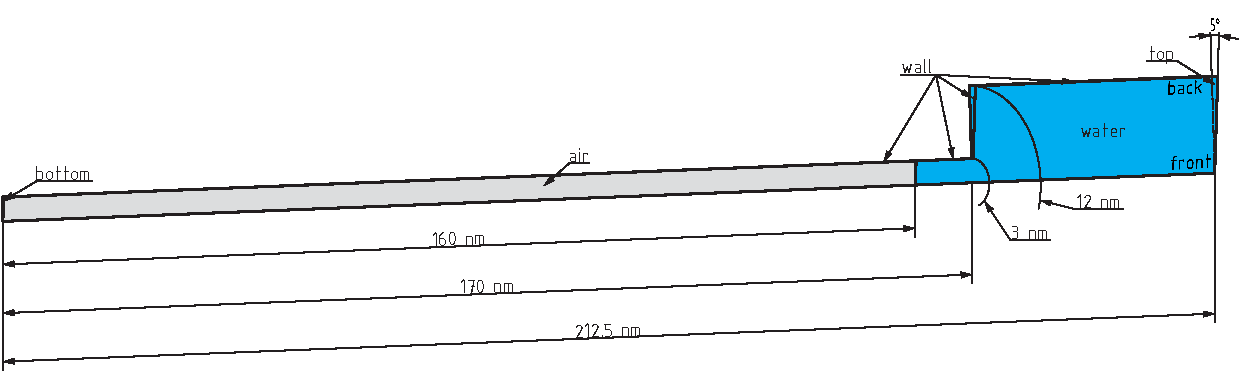
\includegraphics[width=.95\textwidth]{Pictures/Cap_5DEG.pdf}
    \caption{Schematic of used Capillary}
    \label{fig: Capillary Geometry}
\end{figure}
As already indicated in the picture, not the entire capillary is simulated, but only a segment of the capillary, called a \textit{wedge}. It is assumed that the flow in the capillary is axisymmetric, which greatly simplifies the simulation in that fewer elements are needed for discretization, as in this case only a $5^{\circ}$ segment of the capillary is simulated. A necessary condition for simulating the wedge is that it may only have one element in the radial direction. The discretization of the geometry was chosen so that the elements have an edge length of $0.2nm$. To create the \texttt{blockMeshDict} file, a python script was created that creates a file based on the capillary diameter and length with the designations of the surfaces shown in Figure \ref{fig: Capillary Geometry}.

\section{Boundary Conditions}
In Figure \ref{fig: Capillary Geometry}, in addition to the geometry, the surfaces that were provided with boundary conditions are also named. The \texttt{front} and \texttt{back} surfaces are opposing surfaces of the wedge and must therefore receive corresponding boundary conditions. The \texttt{wall} surfaces are impenetrable surfaces, and the \texttt{top} and \texttt{bottom} surfaces are surfaces through which a flow is permitted.
The essential boundary conditions on the wall are listed in Table \ref{tab: BoundaryConditions_wall}.

\begin{table}[h]
    \centering
    \caption{Relevant boundary conditions for the wall}
    \label{tab: BoundaryConditions_wall}
    \begin{tabular}{lll}
        Parameter & Value \\ \hline
        Order parameter $C$ & \texttt{equilibriumPhaseContactAngle} \\
        Equilibrium contact angle $\theta_{\mathrm{e}}$ & $15^{\circ}$, $45^{\circ}$, $75^{\circ}$ \\
        Chemical potential $\phi$ & \texttt{zeroGradient} \\
        Velocity $\mathbf{u}$ & $\mathbf{u_{\mathrm{w}}} = 0$ \\
        Pressure $p$ & \texttt{fixedFluxPressure} \\
    \end{tabular}
\end{table}
For the order parameter $C$, the equilibrium boundary condition is assumed, and the equilibrium contact angle for each of the three simulations with this geometry is given as $15^{\circ}$, $45^{\circ}$, and $75^{\circ}$. For further simulations, in addition to the mentioned equilibrium condition \texttt{equilibriumPhaseContactAngle}, it was also assumed that there is an imbalance according to \ref{sec: nonEquiBC}. For the simulations, the boundary condition must be changed to \texttt{outOfEquilibriumPhaseContactAngle}, and a value for $\Gamma_{\mathrm{w}}$ must be specified.
The gradient of the chemical potential on the wall is set to zero, as is the velocity of the wall. The boundary condition for the pressure is chosen with \texttt{fixedFluxPressure} so that the pressure gradient is adjusted in such a way that the mass flow at the boundary matches the given velocity on the wall.
At the inlet or outlet of the capillary, a \texttt{zeroGradient} boundary condition also applies, and a pressure of $0$ Pa.

\section{Material Properties}
For the simulation, water and air at $25^{\circ}$ Celsius are assumed as the medium, among other things. This results in the material properties shown in Table \ref{tab:physicalProperties_CaseSetup}.
\begin{table}[h]
    \centering
    \caption{Physical properties}
    \label{tab:physicalProperties_CaseSetup}
    \begin{tabular}{lll}
        Fluid & Density $\frac{kg}{m^3}$ & Kinematic viscosity $\frac{m^2}{s}$ \\ \hline
        Water & $1000$ & $1.00E-06$ \\
        Air & $1$ & $1.00E-05$ \\
    \end{tabular}
\end{table}
The surface tension for a water-air interface at $25^{\circ}$ Celsius is given as \(0.072 N/m\). The interface thickness \( \epsilon \) was chosen to be approximately \(1.7 nm\) \cite{bagheriInterfacialRelaxationCrucial2022}, corresponding to the physical interface thickness.


\section{Simulation Parameters}
The mobility ($\kappa$) is a factor in the phase-field simulation that is difficult to determine. Jacqmin \cite{jacqmin1999CalculationTwoPhaseNavier} suggested an asymptotic behavior for \( \kappa \) of 
\begin{equation}
    \kappa = \mathcal{O}(\epsilon^{\delta})
\end{equation}
and showed that \( 1 \leq \delta < 2 \). Unfortunately, there is currently no concrete method for calculating mobility. Therefore, various simulations were conducted to determine a suitable value. The same applies to the wall relaxation factor $\Gamma_{\mathrm{w}}$. The fact that these parameters are phenomenological makes their prediction challenging, and there are only recommendations available.
For this work, a value of \( \kappa = 1.6 \times 10^{-18} \) was used. For the wall relaxation factor $\Gamma_{\mathrm{w}}$, a value of \( \Gamma_{\mathrm{w}} = 5 \times 10^{12} \) was assumed. \todo{CHECK}

Due to initial problems in post-processing, the simulation was conducted without adaptive mesh refinement.
The simulation was initialized with a planar interface, and for the order parameter, an interface profile according to Equation \ref{eq: InterfactialNormalDirProfile} was initialized using the \texttt{funkySetFields} method.

The viscosity model of the simulation is carried out using the \texttt{blended} method. In this approach, the \texttt{arithmetic} and \texttt{harmonic} models are combined using a blending factor.


\section{Evaluation Methods}
For the evaluation of the simulation, the software \texttt{paraview} was used, among other tools. All images of the simulation were generated using this software. However, the evaluation and representation of derived or calculated quantities in diagrams were produced using the Python library \texttt{Matplotlib}. A script was developed to collect the results from the function objects and, if necessary, to perform calculations with them.

With the help of \textit{function objects}, data can be collected during the ongoing simulation. \texttt{phaseFieldFoam} provides several functions for reading out the simulation, which are also used here. These have to be integrated and configured in the \texttt{controlDict} file.

For instance, to analyze the viscous forces acting within the water column, we need the total viscous dissipation force in that water column, which is exported via such function objects. We obtain this by integrating the divergence of the viscous stress tensor $\tau$ from Equation \ref{eq: NSEChanged} over the domain:
\begin{equation}
    \mathrm{F}_{\mathrm{visc}}^{\mathrm{total}} = \int_{\Omega} \mathrm{f}_{\mathrm{visc}}^{\mathrm{total}} dV = \int_{\Omega} \nabla \cdot \tau dV.
\end{equation}

